% Air Pollution -- a self-contained academic Beamer recipe.
% Compile twice with pdfLaTeX. All example content is methodological, not evidence.
\documentclass[aspectratio=169,11pt]{beamer}
\geometry{paperwidth=28.444cm,paperheight=16cm}
\usepackage[T1]{fontenc}
\usepackage{lmodern,ebgaramond,amsmath,amssymb,microtype,tikz}
\usetikzlibrary{calc}
\renewcommand{\rmdefault}{lmr}
\renewcommand{\familydefault}{\rmdefault}
\usefonttheme{professionalfonts}
\definecolor{ink}{HTML}{183B39}
\definecolor{body}{HTML}{293D3B}
\definecolor{muted}{HTML}{60716B}
\definecolor{paper}{HTML}{F7F8F3}
\definecolor{mist}{HTML}{DBE4DD}
\definecolor{copper}{HTML}{A75C3B}
\setbeamercolor{normal text}{fg=body,bg=paper}
\setbeamercolor{structure}{fg=ink}
\setbeamercolor{alerted text}{fg=copper}
\setbeamercolor{background canvas}{bg=paper}
\setbeamerfont{normal text}{size=\fontsize{18}{25}\selectfont}
\setbeamerfont{frametitle}{family=\fontfamily{EBGaramond-TLF}\selectfont,series=\bfseries,size=\fontsize{29}{34}\selectfont}
\setbeamerfont{title}{family=\fontfamily{EBGaramond-TLF}\selectfont,series=\mdseries,size=\fontsize{56}{60}\selectfont}
\setbeamersize{text margin left=1.8cm,text margin right=1.8cm}
\setbeamertemplate{navigation symbols}{}
\setbeamertemplate{itemize item}{\raisebox{0.3ex}{\color{copper}\rule{5pt}{5pt}}}
\setbeamerfont{itemize/enumerate body}{size=\fontsize{18}{25}\selectfont}
\newcommand{\eyebrow}[1]{{\sffamily\fontsize{11}{14}\selectfont\color{muted}\MakeUppercase{#1}}}
\newcommand{\heading}[1]{{\fontfamily{EBGaramond-TLF}\selectfont\fontsize{26}{31}\selectfont\color{ink}#1}}
\newcommand{\sourcenote}[1]{\par\vspace{0.35cm}{\sffamily\fontsize{11}{15}\selectfont\color{muted}#1\par}}
\newcommand{\spaceditems}{\setlength{\itemsep}{0.8cm}}
\newcommand{\chapterlabel}{Research framework}
\setbeamertemplate{frametitle}{%
  \vspace{0.65cm}\eyebrow{Air pollution\enspace /\enspace\chapterlabel}\par
  \vspace{0.32cm}{\usebeamerfont{frametitle}\color{ink}\insertframetitle\par}
  \vspace{0.22cm}{\color{mist}\rule{\textwidth}{0.65pt}}\vspace{0.2cm}
}
\setbeamertemplate{footline}{%
  \begin{beamercolorbox}[wd=\paperwidth,ht=0.65cm,dp=0.35cm,leftskip=1.8cm,rightskip=1.8cm]{normal text}
    \eyebrow{\insertshortauthor\quad /\quad Air pollution}\hfill
    {\sffamily\fontsize{11}{12}\selectfont\color{muted}\insertframenumber\ /\ \inserttotalframenumber}
  \end{beamercolorbox}
}
% Deterministic particles: a visual metaphor, never a measurement or a map.
\newcommand{\atmosphere}{%
  \begin{tikzpicture}[remember picture,overlay]
    \fill[mist] ([xshift=-10cm]current page.north east) rectangle (current page.south east);
    \foreach \i in {1,...,210}{
      \pgfmathsetmacro{\xx}{mod(\i*73,101)/101*8.7}
      \pgfmathsetmacro{\yy}{mod(\i*47,103)/103*13.8}
      \pgfmathsetmacro{\rr}{0.025+mod(\i*13,11)*0.007}
      \pgfmathsetmacro{\op}{0.12+0.45*(1-\yy/13.8)}
      \fill[ink,opacity=\op] ([xshift=-\xx cm-0.6cm,yshift=\yy cm+1cm]current page.south east) circle (\rr cm);
    }
    \draw[copper,line width=1pt] ([xshift=-10.7cm,yshift=3.3cm]current page.south east) -- ([xshift=-0.9cm,yshift=3.3cm]current page.south east);
  \end{tikzpicture}
}
\title[Air Pollution]{Air Pollution}
\subtitle{Exposure, evidence, and environmental policy}
\author[Presenter Name]{Presenter Name}
\institute{Department / Institution}
\date{Research seminar}
\begin{document}
\usebeamerfont{normal text}

% 01 / Cover
\begin{frame}[plain]
  \atmosphere
  \begin{minipage}[c][12.2cm][c]{15cm}
    \eyebrow{Environmental economics\quad /\quad Research seminar}\par
    \vspace{1.25cm}
    {\usebeamerfont{title}\color{ink}\inserttitle\par}
    \vspace{0.6cm}
    \insertsubtitle\par
    \vspace{1.5cm}
    {\color{copper}\rule{1.5cm}{1.5pt}}\par\vspace{0.45cm}
    \insertauthor\par
    \sourcenote{\insertinstitute\quad /\quad\insertdate}
  \end{minipage}
\end{frame}

% 02 / Motivation
\begin{frame}{Begin with a precise exposure question}
  \begin{itemize}\spaceditems
    \item Name the pollutant and its measurement unit.
    \item Define the population and the exposure window.
    \item Select an outcome with a clear interpretation.
    \item State the policy comparison of interest.
  \end{itemize}
  \vspace{0.6cm}
  \sourcenote{Template example: replace this research outline with your study and citations.}
\end{frame}

% 03 / Research question
\begin{frame}{Make the comparison explicit}
  \vspace{0.4cm}
  \begin{center}
    \heading{How does a change in exposure affect outcomes?}\par
    \vspace{1.2cm}
    
\begin{tikzpicture}
      \draw[mist,line width=1pt] (0,0) -- (21,0);
      \foreach \x/\n/\t/\d in {3.5/01/Exposure/Pollutant and time window,10.5/02/Population/People and places at risk,17.5/03/Outcome/Measure and follow-up}{
        \node[text=copper,font=\sffamily\fontsize{12}{15}\selectfont] at (\x,0.55) {\n};
        \node[text=ink,font=\bfseries] at (\x,-0.75) {\t};
        \node[text=muted,font=\fontsize{15}{20}\selectfont] at (\x,-1.65) {\d};
      }
    \end{tikzpicture}
  \end{center}
  \vspace{0.5cm}
\end{frame}

% 04 / Section divider
\begin{frame}[plain]
  \atmosphere
  \begin{minipage}[c][12cm][c]{15cm}
    \eyebrow{01\quad /\quad Research design}\par\vspace{1cm}
    {\usebeamerfont{title}\color{ink}From exposure\\to evidence\par}
    \vspace{0.85cm}
    Measurement. Comparison. Interpretation.\par
    \vspace{1.25cm}{\color{copper}\rule{1.5cm}{1.5pt}}
  \end{minipage}
\end{frame}

% 05 / Measurement
\renewcommand{\chapterlabel}{Measurement}
\begin{frame}{Align exposure with people and time}
  \begin{itemize}\spaceditems
    \item Match pollution measures to a defined location.
    \item Document monitor coverage and missing records.
    \item Align weather controls with the exposure window.
    \item Report aggregation rules and sample restrictions.
  \end{itemize}
  \vspace{0.6cm}
  \sourcenote{Data sources, geographic units, and sample dates belong here.}
\end{frame}

% 06 / Equation
\renewcommand{\chapterlabel}{Identification}
\begin{frame}{An equation makes the estimand visible}
  \begin{center}
    \vspace{0.15cm}
    \[
      Y_{it}=\underbrace{\alert{\beta}}_{\text{target}}\,P_{it}
      +X_{it}'\gamma+\alpha_i+\lambda_t+\varepsilon_{it}
    \]
  \end{center}
  \vspace{0.4cm}
  \begin{itemize}\setlength{\itemsep}{0.5cm}
    \item $P_{it}$ measures exposure for unit $i$ at time $t$.
    \item $\alpha_i$ and $\lambda_t$ absorb unit and time effects.
    \item A causal interpretation needs a credible design.
  \end{itemize}
  \sourcenote{Illustrative specification only; adapt controls and inference to the actual design.}
\end{frame}

% 07 / Identification checks
\begin{frame}{State what makes the comparison credible}
  \begin{itemize}\spaceditems
    \item Describe the source of exposure variation.
    \item Explain the identifying assumption in plain language.
    \item Show diagnostics that can challenge the design.
    \item Discuss remaining threats to interpretation.
  \end{itemize}
  \vspace{0.6cm}
  \sourcenote{Choose diagnostics for the actual design; fixed effects alone do not establish causality.}
\end{frame}

% 08 / Figure style (schematic; deliberately no empirical estimates)
\renewcommand{\chapterlabel}{Visual evidence}
\begin{frame}{Give each figure one message}
  \begin{center}
    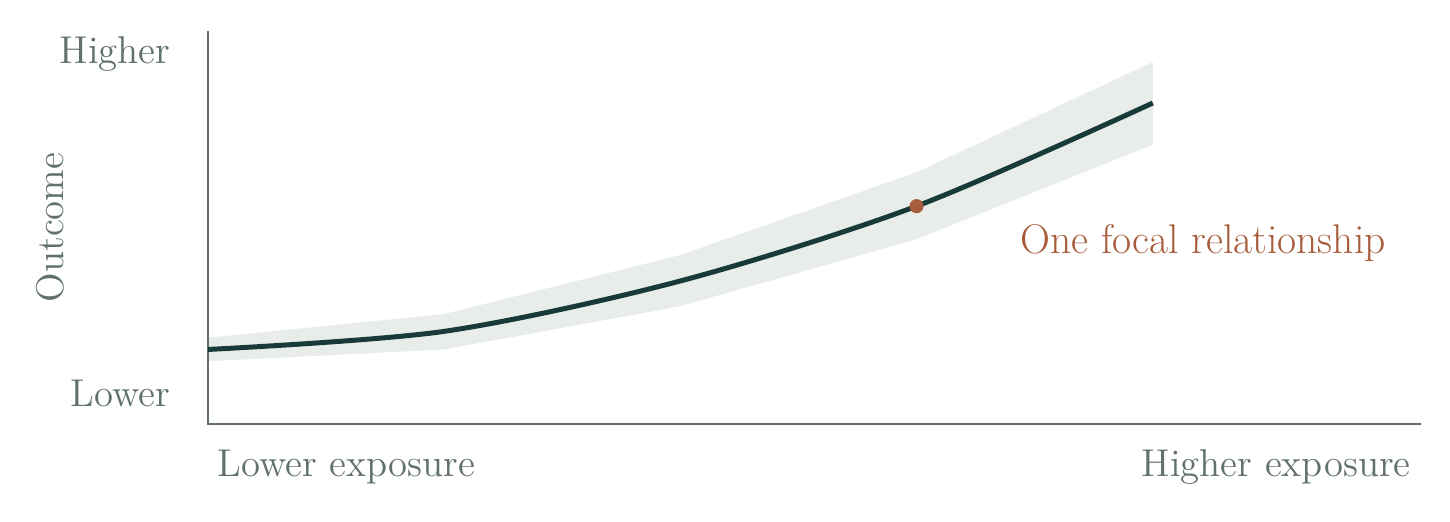
\begin{tikzpicture}[x=1cm,y=1cm]
      \fill[mist,opacity=0.65] (0,1.1) -- (3,1.4) -- (6,2.15) -- (9,3.2) -- (12,4.6)
        -- (12,3.55) -- (9,2.35) -- (6,1.5) -- (3,0.95) -- (0,0.8) -- cycle;
      \draw[muted,line width=0.7pt] (0,5) -- (0,0) -- (15.4,0);
      \draw[ink,line width=1.8pt] plot[smooth] coordinates {(0,0.95) (3,1.18) (6,1.82) (9,2.77) (12,4.08)};
      \fill[copper] (9,2.77) circle (0.09);
      \node[anchor=west,text=copper,font=\fontsize{15}{20}\selectfont] at (10.2,2.3) {One focal relationship};
      \node[anchor=east,text=muted,font=\fontsize{14}{18}\selectfont] at (-0.35,4.7) {Higher};
      \node[anchor=east,text=muted,font=\fontsize{14}{18}\selectfont] at (-0.35,0.4) {Lower};
      \node[text=muted,font=\fontsize{14}{18}\selectfont,rotate=90] at (-2,2.5) {Outcome};
      \node[anchor=north west,text=muted,font=\fontsize{14}{18}\selectfont] at (0,-0.2) {Lower exposure};
      \node[anchor=north east,text=muted,font=\fontsize{14}{18}\selectfont] at (15.4,-0.2) {Higher exposure};
    \end{tikzpicture}
  \end{center}
  \sourcenote{Schematic only: the curve and shaded envelope are layout examples, not estimates or confidence intervals.}
\end{frame}

% 09 / Results reporting
\renewcommand{\chapterlabel}{Interpretation}
\begin{frame}{Report magnitude together with uncertainty}
  \begin{itemize}\spaceditems
    \item Express the estimate in meaningful exposure units.
    \item Show an interval and explain the inference method.
    \item Compare the effect with the baseline outcome mean.
    \item Separate the estimate from the policy extrapolation.
  \end{itemize}
  \vspace{0.6cm}
  \sourcenote{Insert verified results and citations. This recipe supplies no empirical findings.}
\end{frame}

% 10 / Closing
\begin{frame}[plain]
  \atmosphere
  \begin{minipage}[c][12cm][c]{15cm}
    \eyebrow{Air pollution\quad /\quad Discussion}\par\vspace{1cm}
    {\usebeamerfont{title}\color{ink}Clear questions.\\Credible evidence.\par}
    \vspace{0.9cm}
    Bring the discussion back to the estimand.\par
    \vspace{1.2cm}{\color{copper}\rule{1.5cm}{1.5pt}}\par
    \sourcenote{\insertauthor\quad /\quad name@example.edu}
  \end{minipage}
\end{frame}
\end{document}
